\section*{Problema 2}
\textbf{Sea el siguiente spline cúbico:}
\begin{equation*}
	f(x) = \begin{cases}
		f_0(x)= ax^3+bx^2+c(x-1) & -1\leq x \leq 0 \\
		f_1(x) = d(x-1)^2 +ex    & 0\leq x \leq 1
	\end{cases}
\end{equation*}
\begin{enumerate}
	\item \textbf{Determina los valores de $a,b,c,d$ y $e$ si $f$ interpola $f(-1)=-4$ y $f(1)=1$.}

	      Se plantea que $f,f'$ y $f''$ es continua, entonces esta debera cumplir la siguiente condición:

	      \begin{align*}
		      f_0(0)   & = f_1(0)   \\
		      f'_0(0)  & = f'_1(0)  \\
		      f''_0(0) & = f''_1(0)
	      \end{align*}

	      esto es porque $f_0$ y $f_1$  son funciones que comparten $x=0$ en su dominio. Entonces, usando esta condición con las dadas, se obtiene el siguiente sistema de ecuaciones:

	      \begin{align*}
		      -a+b-2c & = -4 \\
		      e       & = 1  \\
		      c+d     & = 0  \\
		      b-d     & =0   \\
		      c+2d-e  & = 0
	      \end{align*}

	      Por lo tanto, se obtiene que la solución es la siguiente:

	      \begin{align*}
		      a = 7 \qquad & b = 1 \qquad c= -1 \\
		      d = 1        & \qquad e=1
	      \end{align*}

	      En la figura \ref{fig:problema02a} se muestra la función $f$ con los parámetros obtenidos.

	      \begin{figure}[H]
		      \centering
		      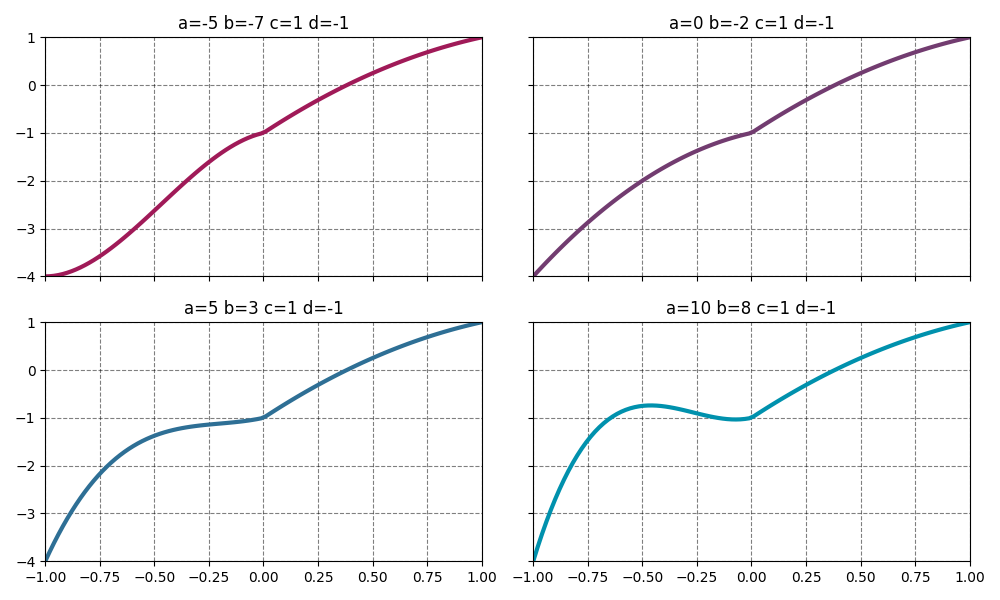
\includegraphics[width=14cm]{Graphics/problema02a.png}
		      \caption{Función $f$ con varios parámetros.}
		      \label{fig:problema02a}
	      \end{figure}

	\item \textbf{Determina los valores de $a,b,c,d$ y $e$ si $f$ interpola $f'(-1)=6$ y $f(1)=-1$.}

	      Calculando la primer derivada de $f$, se obtiene lo siguiente:

	      \begin{equation*}
		      f'(x) = \begin{cases}
			      f'_0(x)= 3ax^2+2bx+c & -1\leq x \leq 0 \\
			      f'_1(x) = 2d(x-1) +c & 0\leq x \leq 1
		      \end{cases}
	      \end{equation*}

	      Como $f'$ debe de ser continua, entonces $f'_0(0) = f'_1(0)$. Contemplando las condicones dadas, entonces se obtiene el siguiente sistema de ecuaciones:

	      \begin{align*}
		      3a -2b +c & =6   \\
		      e         & = -1 \\
		      c+d       & = 0  \\
		      b-d       & = 0  \\
		      c+2d -e   & = 0
	      \end{align*}

	      Por lo tanto, se obtiene que la solución del sistema de ecuaciones es:

	      \begin{align*}
		      a  = 1 \qquad & b=-1 \qquad c =1 \\
		      d = -1        & \qquad e =-1
	      \end{align*}

	      En la figura \ref{fig:problema02b} se muestra la función $f$ con los parámetros obtenidos.
	      \begin{figure}[H]
		      \centering
		      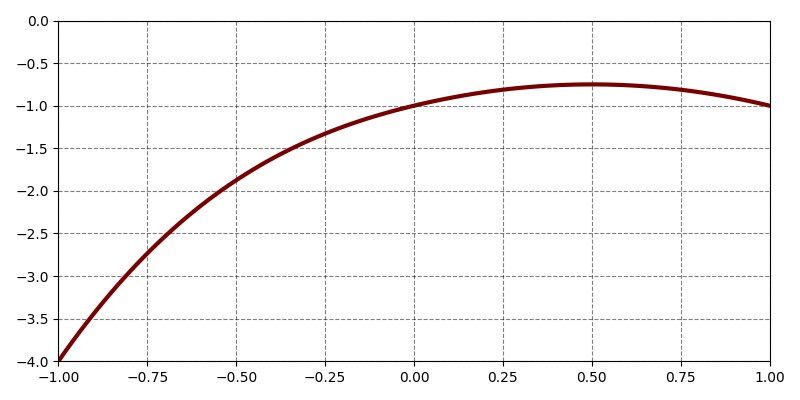
\includegraphics[width=14cm]{Graphics/problema02b.png}
		      \caption{Función $f$ con varios parámetros.}
		      \label{fig:problema02b}
	      \end{figure}
\end{enumerate}
\pagebreak
